\pagebreak
\subsection{Use Cases}
\centerline{
	\vspace{2cm}
		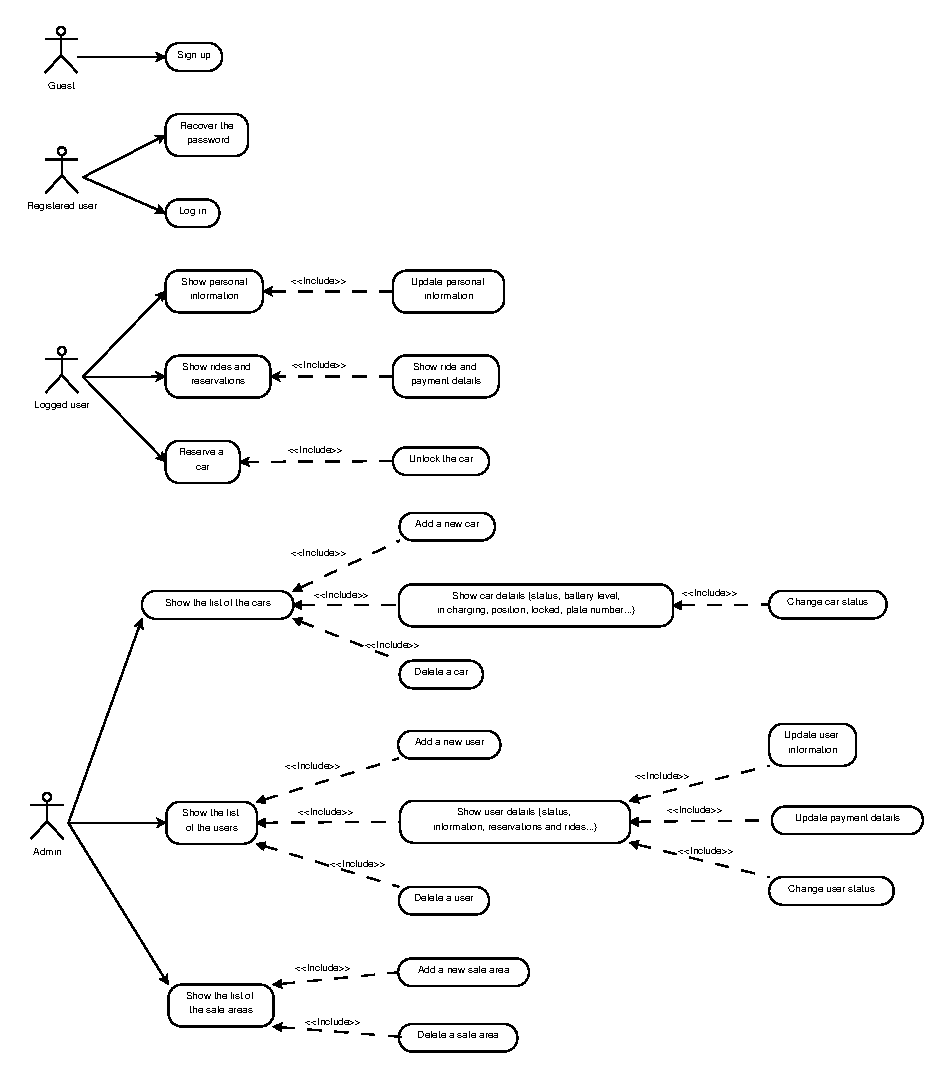
\includegraphics{UseCaseDiagram.eps}}



\pagebreak
In this paragraph we are going to identify and describe the most important use cases of ``PowerEnjoy'' web application.
Based on the scenarios defined in the previous chapter, we can derive some significant use cases:
\begin{enumerate}
	\item Registration
	\item Log in
	\item Recover the password
	\item Reserve a car
	\item Unlock the reserved car
	\item End the ride
	\item Expired reservation
	\item Payment not successful
	\item Update personal information
	\item Show the details of the ride
	\item Add new cars
	\item Delete a safe area
\end{enumerate}

% Definition of UseCase environment
\newtoggle{exception}
\newenvironment{UseCase}[5]{
	\paragraph{Partecipating actors:} #1
	\paragraph{Entry condition:} #2
	\paragraph{Flow of events:}
	\begin{itemize} 
		#3 
	\end{itemize}
	\paragraph{Exit condition:} #4
	\iftoggle{exception}{
		\paragraph{Exceptions:}
		\begin{itemize}
			#5
		\end{itemize}
	}{
	}
}{}

\newcommand{\Event}[1]{
	\item #1
}

\newcommand{\Exc}[2]{
	\item \textbf{#1:} #2
	
}


\subsubsection{Registration}
\toggletrue{exception}
\begin{UseCase}
	{Guest: a guest is whoever visits the website}
	{This use case starts when the guest access the homepage of the web application and clicks on ``\textit{Sign up}''.}
	{
		\Event{The guest clicks on ``\textit{Sign up}''}
		\Event{The guest fills out the form entering all required information:
			\begin{itemize}
				\item name
				\item surname
				\item address
				\item e-mail
				\item mobile phone number
				\item driving license number
				\item credit card number
		\end{itemize}}
		\Event{The guest checks the checkbox ``\textit{I have read and agree to PowerEnJoy Terms of Use and Privacy Policy.}''}
		\Event{The guest clicks on ``\textit{Confirm}''}
		\Event{The system verifies that the user isn't already registered}
		\Event{The system verifies that the user's credit card is valid}
		\Event{The system verifies that the user's driving license is valid}
		\Event{The system stores the new data in the users database}
		\Event{The system sends the user an e-mail containing his/her credentials (username and password)}
		\Event{The system displays a confirmation message, informing the new user that the registration has been successfully completed}
		\Event{The system shows the new user the log in page}
	}
	{This use case terminates when the registration is successfully completed and the new user receives the mail with his/her credentials.}
	{
		\Exc{The guest is already a registered user}{if this exception occurs, the system displays the error message: ``\textit{ERROR: you are already registered!}'' and the application goes back to the page where the registration form is shown.}
		\Exc{The user's credit car isn't valid}{if this exception occurs, the system displays the error message: ``\textit{ERROR: your credit card is not valid!}'' and the application goes back to the page where the registration form is shown.}
		\Exc{The user's driving license is not valid}{if this exception occurs, the system displays the error message: ``\textit{ERROR: your driving license is not valid!}'' and the application goes back to the page where the registration form is shown.}
		\Exc{The user doesn't fill all the fields in the registration form}{if this exception occurs, the system displays the error message: ``\textit{ERROR: all the fields has to be filled!}'' and the application goes back to the page where the registration form is shown.}
	}
\end{UseCase}


\subsubsection{Log in}
\begin{UseCase}
	{Registered user: a registered user is a guest that has already signed up.}
	{This use case starts when the registered user, that has already received the e-mail with his/her credentials, clicks on ``\textit{Log in}'' from the homepage of the website.}
	{
		\Event{The registered user clicks on ``\textit{Log in}''}
		\Event{The registered user enters his/her email}
		\Event{The registered user enters his/her password}
		\Event{The registered user clicks on ``\textit{Confirm}''}
		\Event{The system checks the inserted username}
		\Event{The system checks the inserted password}
		\Event{The system shows the user's personal profile page}
	}
	{This use case terminates when the log in is successfully completed and the new user access his/her personal area.}
	{
		\Exc{The inserted email is incorrect}{if this exception occurs, the system displays the error message: ``\textit{ERROR: the inserted email is wrong!}'' and the application goes back to the log in page.}
		\Exc{The inserted password is incorrect}{if this exception occurs, the system displays the error message: ``\textit{ERROR: the inserted password is wrong!}'' and the application goes back to the log in page}
	}
\end{UseCase}

\subsubsection{Recover the password}
\togglefalse{exception}
\begin{UseCase}
	{Registered user: a registered user is a guest that has already signed up.}
	{This use case starts when the user forgot the password and clicks on ``\textit{Send a new password}'' from the log in page.}
	{
		\Event{The registered user is on the log in page and clicks on ``\textit{Send a new password}''}
		\Event{The system sends the user an e-mail with the new password}
		\Event{The system displays a confirmation message}
		\Event{The system displays the log in page}
		\Event{The user receives the e-mail with the new password}
	}
	{This use case terminates when the user receives the new password by e-mail.}{}
\end{UseCase}

\subsubsection{Reserve a car}
\toggletrue{exception}
\begin{UseCase}
	{Registered user: a registered user is a guest that has already signed up.}
	{This use case starts when, after logging in, the registered user clicks on ``\textit{Reserve a car}'' from his/her personal profile page.}
	{
		\Event{The registered user clicks on ``\textit{Reserve a car}''}
		\Event{The system shows the reservation form}
		\Event{The user selects where to search the car: choosing if use his/her current location or a specified address (in this case he/she also has to write an address)}
		\Event{The user selects a maximum distance for the car research}
		\Event{The user clicks on ``\textit{Search cars}''}
		\Event{The system searches available cars within the maximum distance indicated from the given location}
		\Event{The system shows the list of available cars}
		\Event{The user selects one of the cars in the list}
		\Event{The user clicks on ``\textit{Reserve}''}
		\Event{The system changes the status of the car from ``\textit{available}'' to ``\textit{reserved}''}
		\Event{The system displays a confirmation message containing the details of the reservation (time of the reservation, license plate, position, distance from the given location \ldots)}
		\Event{The system displays the user's personal profile page}
	}
	{This use case terminates when the confirmation message is shown and the user is redirected on his/her personal profile page.}
	{
		\Exc{The user doesn't select a location for the car research}{if this exception occurs, the system displays the error message: ``\textit{ERROR: you have to select a location for the car research!}'' and the application goes back to the page where the reservation form is shown.}
		\Exc{The user writes an inexistent address}{if this exception occurs, the system displays the error message: ``\textit{ERROR: the inserted address doesn't exist!}'' and the application goes back to the page where the reservation form is shown.}
		\Exc{The user writes an invalid value for the maximum distance}{if this exception occurs, the system displays the error message: ``\textit{ERROR: the inserted distance isn't valid!}'' and the application goes back to the page where the reservation form is shown.}
		\Exc{There aren't cars in the selected area}{if this exception occurs, the system displays the error message: ``\textit{ERROR: there are no cars in the selected area! Please change the maximum distance or the selected location.}'' and the application goes back to the page where the reservation form is shown.}
	}
\end{UseCase}

\subsubsection{Unlock the reserved car}
\begin{UseCase}
	{Registered user: a registered user is a guest that has already signed up.}
	{This use case starts when a registered user who has already reserved a car wants to unlock it, so logs in the application.}
	{
		\Event{The system displays the user's personal profile page}
		\Event{The user clicks on ``\textit{Unlock the reserved car}''}
		\Event{The system checks the distance between the user and the reserved car}
		\Event{The system change the status of the car from ``\textit{reserved}'' to ``\textit{in use}''}
		\Event{The system unlocks the car}
		\Event{The user gets on the car in less than ten minutes}
	}
	{This use case terminates when the system unlocks the car and the user gets in.}
	{
		\Exc{The user is at more than 3 meters from the car}{if this exception occurs, the system displays the error message: ``\textit{ERROR: you are too far from the car to unlock it! Please go next to the reserved car.}'' and the application shows the user's personal profile page.}
		\Exc{The user doesn't gets on the car in less than ten minutes}{if this exception occurs, the system locks the car and the ride is considered ended.}
	}
\end{UseCase}

\subsubsection{End the ride}
\togglefalse{exception}
\begin{UseCase}
	{Registered user: a registered user is a guest that has already signed up.}
	{This use case starts when the car is parked and the user and all eventual passengers exit the car.}
	{
		\Event{The user parks and turns off the car}
		\Event{The user and eventual passengers exit the car}
		\Event{The system locks the car}
		\Event{The system waits five minutes}
		\Event{The system checks the location}
		\Event{The system checks the level of the battery}
		\Event{The system checks if the power grid is plugged}
		\Event{The system calculates the total to be paid}
		\Event{The system charges the user the cost of the ride}
		\Event{The system changes the status of the car from ``\textit{in use}'' to ``\textit{available}'' or ``\textit{unavailable}'', based on  car conditions}
		\Event{The system sends the user an e-mail containing all the details of the ride (total cost, discounts, fees, duration, starting location, ending location\ldots)}
		\Event{The user receives the e-mail}
	}
	{This use case terminates when the user receives the e-mail containing the details of his last ride.}{}
\end{UseCase}

\subsubsection{Expired reservation}
\begin{UseCase}
	{Registered user: a registered user is a guest that has already signed up.}
	{This use case starts when an hour has passed from when the user reserved a car and he/she hasn't already unlocked the car.}
	{
		\Event{After an hour from the reservation, the system changes the status of the car from ``\textit{reserved}'' to ``\textit{available}''}
		\Event{The system imposes a charge of 1 euro to the user}
	}
	{This use case terminates when the status of the car is changed into ``\textit{available}''}{}
\end{UseCase}

\subsubsection{Payment not successful}
\begin{UseCase}
	{Registered user: a registered user is a guest that has already signed up.}
	{This use case starts when the automatic payment fails.}
	{
		\Event{The automatic payment fails and the external service notifies the system.}
		\Event{The systam change the status of the user's account from ``\textit{active}'' to ``\textit{insolvent}''}
		\Event{The system sends the user an e-mail telling to get in touch with the costumer care}
		\Event{The user receive the e-mail}
	}
	{This use case terminates when the user receive the e-mail.}{}
\end{UseCase}

\subsubsection{Update personal information}
\toggletrue{exception}
\begin{UseCase}
	{Registered user: a registered user is a guest that has already signed up.}
	{This use case starts when a registered user is on his/her personal profile page and clicks on ``\textit{Personal information}''.}
	{
		\Event{The user clicks on ``\textit{Personal information}''}
		\Event{The system shows the page where the user can visualize his/her personal information}
		\Event{The user clicks on ``\textit{Edit}''}
		\Event{The system shows an input form where the user can make changes}
		\Event{The user updates the information he/she wants in the specific input form}
		\Event{The user clicks on ``\textit{Save changes}''}
		\Event{The system verifies that the user's credit card is valid}
		\Event{The system verifies that the user's driving license is valid}
		\Event{The system stores the new data in the users database}
		\Event{The system shows the page where the user can visualize his/her personal information}
	}
	{This use case terminates when the new data are stored in the users database and the personal information page is shown.}
	{
		\Exc{The user's credit car isn't valid}{if this exception occurs, the system displays the error message: ``\textit{ERROR: your credit card is not valid!}'' and the application goes back to the page where the user can make changes.}
		\Exc{The user's driving license is not valid}{if this exception occurs, the system displays the error message: ``\textit{ERROR: your driving license is not valid!}'' and the application goes back to the page where the user can make changes.}
	}
\end{UseCase}

\subsubsection{Show the details of the ride}
\begin{UseCase}
	{Registered user: a registered user is a guest that has already signed up.}
	{This use case starts when a registered user clicks on ``\textit{My rides}'' from his/her personal profile page.}
	{
		\Event{The registered user clicks on ``\textit{My rides}''}
		\Event{The system shows the page where the user can visualize the list of his/her rides and reservations}
		\Event{The user clicks on the selected ride or reservation}
		\Event{The system shows the specific page of the ride (or reservation) selected containing all the details}
	}
	{This use case terminates when the system visualize the details of the ride (or reservation) selected by the user.}
	{
		\Exc{The user is just registered to the application and he/she has never reserved nor used a ``PowerEnJoy'' electric car}{if this exception occurs, the system show an empty list.}
	}
\end{UseCase}

\subsubsection{Add new cars}
\togglefalse{exception}
\begin{UseCase}
	{Admin: an admin is a person whose task is to manage cars, safe areas, users and other administratos.}
	{This use case starts when an admin logs in.}
	{
		\Event{The admin logs in with his/her credentials}
		\Event{The system shows the administrators page}
		\Event{The administrator clicks on the button ``\textit{Cars}''}
		\Event{The system show the list of all ``PowerEnJoy'' cars}
		\Event{The administrator clicks on ``\textit{Add a new car}''}
		\Event{The system shows the form where the admin can visualize the list of his/her rides and reservations}
		\Event{The system checks and sets the information provided by sensors on the car}
		\Event{The system add the car to the database and show a confirmation message}
	}
	{This use case terminates when the system shows the confirmation message.}{}
\end{UseCase}

\subsubsection{Delete a safe area}
\begin{UseCase}
	{Admin: an admin is a person whose task is to manage cars, safe areas, users and other administratos.}
	{This use case starts when an admin logs in.}
	{
		\Event{The admin logs in with his/her credentials}
		\Event{The system shows the administrators page}
		\Event{The administrator clicks on the button ``\textit{Safe areas}''}
		\Event{The system shows the list of all ``PowerEnJoy'' safe areas and power grid stations}
		\Event{The administrator selects the safe area that has to be deleted and clicks on it}
		\Event{The system shows the details about the selected safe area}
		\Event{The administrator clicks on ``\textit{Delete}''}
		\Event{The system delete the selected safe area from the database and shows a confirmation message}
	}
	{This use case terminates when the system shows the confirmation message.}{}
\end{UseCase}